\subsection{Dynamic Model}

\subsubsection{Sequence Diagrams}
In this section, sequence diagrams have been created from our use cases. We have the following sequence diagrams:\\

\textbf{Sequence Diagram for our CreateTag use case:}\\
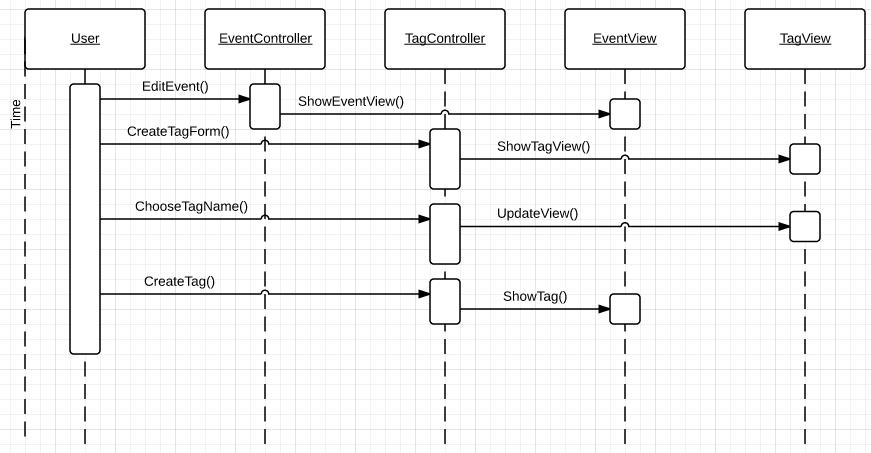
\includegraphics[scale=0.5]{SequenceDiagramUseCaseOne}\\

\textbf{Sequence Diagram for our ChooseTag use case:}\\
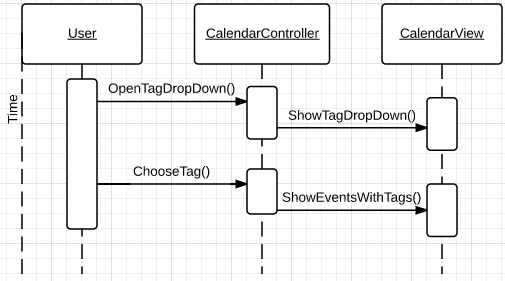
\includegraphics[scale=0.5]{SequenceDiagramUseCaseTwo}\\

\textbf{Sequence Diagram for our GetNotification use case:}\\
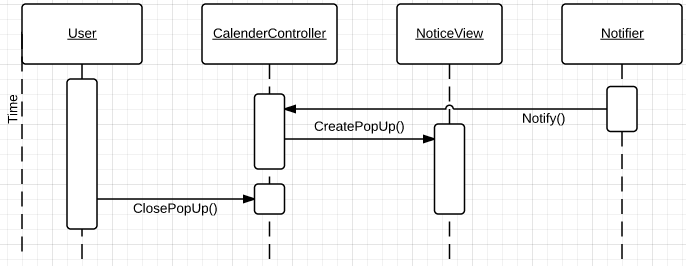
\includegraphics[scale=0.5]{SequenceDiagramUseCaseThree}\\

\newpage
\subsubsection{State Machine Diagrams}
In this section, state machine diagrams have been created for some of the objects described in the initial object analysis. Some of the diagrams have states where they wait for the other object to respond. In these cases the state will be named as following: ObjectNameState.\\

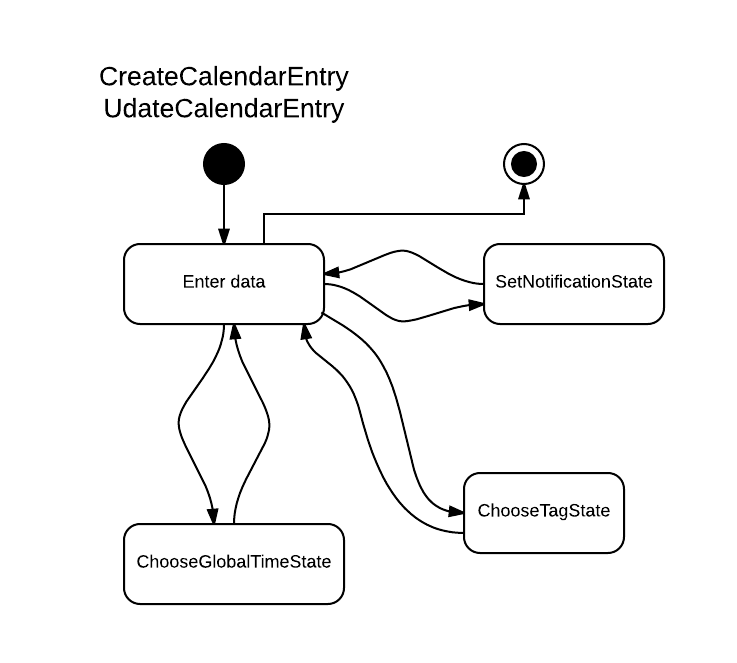
\includegraphics[scale=0.5]{CreateUpdateEntry-StateDiagram}

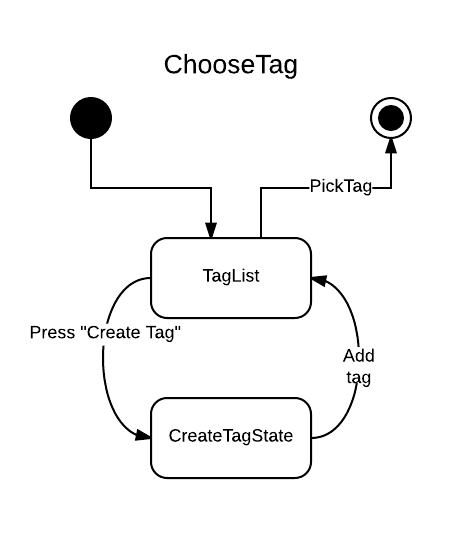
\includegraphics[scale=0.6]{ChooseTag-StateDiagram}

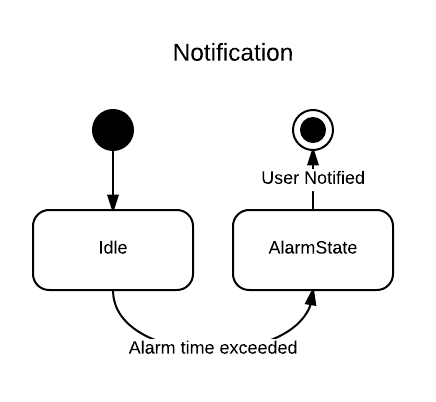
\includegraphics[scale=0.6]{Notification-StateDiagram}

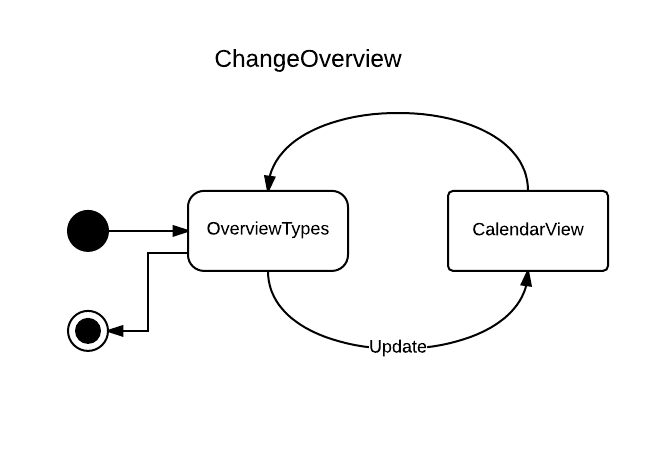
\includegraphics[scale=0.5]{ChangeOverview-StateDiagram}